% !TEX root = thesis.tex
% !TEX encoding = UTF-8
\chapter{チャネル予測モデルの重み更新に向けた補間手法比較}{}
\label{chap:3rd}
\section{はじめに}



\section{CSIの時系列補間手法}
\label{sec:interpolation_methods}
本節では,予測を継続したまま欠損する正解ラベルを扱うための補間手法を説明する.チャネル予測モデル運用時には,予測スロットにおいて\(\bm{H}_t\)が欠損するため,後続スロットで得られる推定値から補間値\(\widetilde{\bm{H}}_t\)を算出し,更新用サンプル生成に用いる.
補間は時間方向に対して行い,各スロットのCSIをフラット化した特徴量ベクトルの各次元に対して適用する.
本論文では,複数の補間手法を比較対象として用いる.以下に示す手法は,補間対象時刻の前後に存在する推定値から\(\widetilde{\bm{H}}_t\)を得るという点が共通である.
補間対象時刻より後に得られる推定値も用いるため,欠損を一方向の外挿として扱う場合に比べて,補間値の推定誤差を抑えられる.

\subsection{線形補間}
最も簡単な基準手法として,補間対象時刻の前後1スロットで得られる推定値の平均を補間値とする.
補間対象時刻を\(t\)とすると,\(\bm{H}_{t-1}\)と\(\bm{H}_{t+1}\)から補間値\(\widetilde{\bm{H}}_t\)を
\begin{equation}
  \widetilde{\bm{H}}_t=\frac{1}{2}\left(\bm{H}_{t-1}+\bm{H}_{t+1}\right)
\end{equation}
として算出する.

\subsection{スプライン補間}
スプライン補間では,補間対象時刻の前後に存在する複数スロットの推定値を用い,時間方向に平滑な曲線で\(\widetilde{\bm{H}}_t\)を算出する.
具体例として,補間対象を\(\bm{H}_3\)とし,近傍として\(\bm{H}_0,\bm{H}_1,\bm{H}_2,\bm{H}_4,\bm{H}_5,\bm{H}_6\)の6点を用いる.
補間対象時刻\(t=3\)からの相対時刻を\(\tau\)とし,\(\tau\)が取り得る値の集合を\(\mathcal{T}=\{-3,-2,-1,1,2,3\}\)と定義する.
すなわち,\(\tau=-3\)は時刻0,\(\tau=1\)は時刻4に対応する.このとき,観測点を
\begin{equation}
  \left\{(\tau,\bm{H}_{3+\tau})\mid \tau\in\mathcal{T}\right\}
\end{equation}
と表す.この観測点を通過する三次スプライン関数\(\bm{s}(\tau)\)を構成し,
\begin{equation}
  \bm{s}(\tau)=\bm{H}_{3+\tau}\quad \tau\in\mathcal{T}
\end{equation}

を満たすように係数を定める.境界条件は自然スプラインとする.これは,観測区間の両端で曲率が0となる条件を課し,端点付近で過度に曲がることを抑える設定である.\(\tau=0\)で評価して

\begin{equation}
  \widetilde{\bm{H}}_3=\bm{s}(0)
\end{equation}
を得る.

\subsection{低次多項式近似}
多項式近似では,時間方向のみに対して低次多項式を当てはめ,補間対象時刻の値を推定して\(\widetilde{\bm{H}}_t\)を算出する.
補間対象を時刻\(t\)とし,補間対象時刻からの相対時刻を\(\tau\)とする.近傍として用いる\(\tau\)の集合を\(\mathcal{T}=\{\tau_1,\ldots,\tau_K\}\)とする.
このとき,\(\tau_i\in\mathcal{T}\)に対応する観測値を\(\bm{H}_{t+\tau_i}\)とし,次数\(d\)の多項式
\begin{equation}
  \bm{p}(\tau)=\sum_{m=0}^{d}\bm{a}_m \tau^m
\end{equation}
により時間方向の変化を近似する.係数\(\{\bm{a}_m\}_{m=0}^{d}\)は最小二乗により
\begin{equation}
  \{\bm{a}_m\}=\arg\min_{\{\bm{a}_m\}}\sum_{i=1}^{K}\left\lVert \bm{H}_{t+\tau_i}-\bm{p}(\tau_i)\right\rVert_2^2
\end{equation}
として推定する.推定後,\(\tau=0\)で評価して補間値を
\begin{equation}
  \widetilde{\bm{H}}_t=\bm{p}(0)=\bm{a}_0
\end{equation}
として得る.

本論文では,多項式の次数\(d\)と近傍点数\(K\)を変化させ,補間精度と更新後の予測精度の関係を比較する.
次数の比較では,\(\mathcal{T}=\{-3,-2,-1,1,2,3\}\)の6点を用い,\(d\in\{2,3,4\}\)を比較する.
近傍点数の比較では,参照信号削減に伴う欠測の周期を\(P=4\)とし,欠測時刻に対応する時刻差を近傍候補から除外する.
具体的には,\(\mathbb{Z}\)を整数集合として,候補集合を
\begin{equation}
  \mathcal{C}=\{\tau\in\mathbb{Z}\mid \tau\neq 0,\ \tau\not\equiv 0\ (\mathrm{mod}\ P)\}
\end{equation}
と定義し,\(\mathcal{C}\)から負の側に\(k_{\mathrm{true}}\)点,正の側に\(k_{\mathrm{true}}\)点を近い順に選び,
\begin{equation}
  \mathcal{T}=\{\tau\in\mathcal{C}\mid \tau<0\}^{k_{\mathrm{true}}}\cup \{\tau\in\mathcal{C}\mid \tau>0\}^{k_{\mathrm{true}}}
\end{equation}
として近傍点集合を構成する.ここで,\(\{\cdot\}^{k_{\mathrm{true}}}\)は絶対値が小さい順に\(k_{\mathrm{true}}\)点を選ぶ演算を表す.
例として,\(k_{\mathrm{true}}=3\)では\(\mathcal{T}=\{-3,-2,-1,1,2,3\}\)となり,\(k_{\mathrm{true}}\)を増やすことで\(\pm 4,\pm 8,\ldots\)を除外しつつ,より遠方の真値点を近傍に含める.

\subsection{ニューラルネットワークによる補間}
ニューラルネットワークを用いた補間では,補間対象時刻を\(t\)とし,補間に用いる時刻差の集合\(\mathcal{T}=\{-3,-2,-1,1,2,3\}\)に対応する推定値を入力として,\(\bm{H}_t\)への回帰を学習する.
\(\bm{H}_{t+\tau}\)をフラット化したベクトルを\(\bm{h}_{t+\tau}\)とし,入力ベクトルを
\begin{equation}
  \bm{x}_t=\left[\bm{h}_{t-3}^{\mathsf{T}},\bm{h}_{t-2}^{\mathsf{T}},\bm{h}_{t-1}^{\mathsf{T}},\bm{h}_{t+1}^{\mathsf{T}},\bm{h}_{t+2}^{\mathsf{T}},\bm{h}_{t+3}^{\mathsf{T}}\right]^{\mathsf{T}}
\end{equation}
と定義する.サンプルごとの振幅差を抑えるため,\(\bm{x}_t\)をRMSで正規化し,
\begin{equation}
  \alpha_t=\sqrt{\frac{1}{\mathrm{dim}(\bm{x}_t)}\left\lVert \bm{x}_t\right\rVert_2^2},\quad
  \bar{\bm{x}}_t=\frac{1}{\alpha_t}\bm{x}_t
\end{equation}
を得る.学習済み補間器を\(g_{\phi}(\cdot)\)とする.ここで,\(g_{\phi}\)の出力は補間対象時刻のCSIをフラット化したベクトルであり,\(\widetilde{\bm{h}}_t\)と表す.補間値は
\begin{equation}
  \widetilde{\bm{h}}_t=\alpha_t\, g_{\phi}(\bar{\bm{x}}_t)
\end{equation}
として算出する.\(\widetilde{\bm{h}}_t\)をスロット\(t\)のCSI行列の形状に戻すことで\(\widetilde{\bm{H}}_t\)を得る.

\subsubsection{補間ニューラルネットワーク}

補間器は,欠損している中心時刻\(t\)のCSI \(\bm{H}_t\)を,その前後の近傍フレームから推定するニューラルネットワークである.
本論文では,context\_size\(=3\)として\(\mathcal{T}=\{-3,-2,-1,1,2,3\}\)の6近傍フレームを用い,それらをフラット化して結合した入力\(\bm{x}_t\in\mathbb{R}^{6F}\)から,中心フレーム1枚分のCSIをフラット化した出力\(\widetilde{\bm{h}}_t\in\mathbb{R}^{F}\)を推定する.
得られた\(\widetilde{\bm{h}}_t\)を行列形状に戻すことで補間値 \(\widetilde{\bm{H}}_t\)を構成する.

\paragraph{MLP補間器}
基本設定の補間器は,全結合層からなるMLPとして実装する.context\_size\(=3\)のときの層構成は以下のとおりである(活性化はReLU).
\begin{itemize}
  \item \(\mathrm{Linear}(6F\rightarrow 2048)\rightarrow \mathrm{ReLU}\)
  \item \(\mathrm{Linear}(2048\rightarrow 1024)\rightarrow \mathrm{ReLU}\)
  \item \(\mathrm{Linear}(1024\rightarrow F)\)
\end{itemize}

\paragraph{RMS正規化(学習・推論で共通)}
チャネル全体のスケール変動に対して学習を安定化させるため,入力\(\bm{x}_t\)のRMSから正規化係数\(\alpha_t\)を計算し,\(\bar{\bm{x}}_t=\bm{x}_t/\alpha_t\)を補間器へ入力する(式(\ref{tab:training_hyperparams})より前で定義した\(\alpha_t\)および\(\bar{\bm{x}}_t\)と同一).
補間器の出力は元スケールへ戻して用い,\(\widetilde{\bm{h}}_t=\alpha_t\,g_{\phi}(\bar{\bm{x}}_t)\)として\(\widetilde{\bm{H}}_t\)を得る.

% \paragraph{3D CNN補間器(オプション)}
% 補間器の選択肢として,3次元畳み込みニューラルネットワーク `InterpolatorCNN3D` も用意する.
% 設定 `--interpolator-model cnn3d` のときに利用され,context\_size\(=3\)(前後3フレームの計6フレーム)に固定される.
% このモデルは,入力CSIをフラット化せずテンソルとして扱い,時間方向(近傍フレーム)と周波数・アンテナ方向の局所相関を3D畳み込みにより抽出して,中心フレームのCSIを回帰する設計である.

% \begin{table}[H]
%   \centering
%   \caption{学習で用いたハイパーパラメータ}
%   \label{tab:training_hyperparams}
%   \begin{tabular}{lccc}
%     \hline
%     フェーズ & エポック数 & バッチサイズ & 学習率 \\
%     \hline
%     予測モデル学習 & 40 & 256 & $10^{-3}$ \\
%     補間モデル学習 & 10 & 128 & $10^{-4}$ \\
%     予測モデルファインチューニング & 20 & 128 & $10^{-4}$ \\
%     \hline
%   \end{tabular}
% \end{table}



\section{シミュレーション}

本節では,補間手法の評価手順について述べた後に,シミュレーションによる評価を行う.

\subsection{地形データとSionnaによるレイトレーシング} \label{subsec:terrain_raytracing} 
本論文で用いるCSI系列はSionna\cite{Makhlouf2025MOCSID}のレイトレーシングにより生成したものである.
 OpenStreetMapから取得した地形データを三次元モデル化し,Sionnaへ入力してCSI系列を生成する.
 白線は端末の移動軌跡であり,赤点は基地局が設置されている位置である.

白線で示される歩行軌道は,現実的な移動経路を生成するためにPRM(Probabilistic Roadmap Method: 確率的ロードマップ法)を用いて生成した.
PRMは複雑な障害物環境における経路計画アルゴリズムであり,ロードマップ構築フェーズと経路探索フェーズの二段階から構成される.

ロードマップ構築フェーズでは,まず移動可能な空間内にランダムにノードを配置する.
各ノードについて鉛直上方にレイを照射し,建物等に衝突した点を屋内と判定して除外することで,屋外のノードのみを抽出する.
次に,KDTreeを用いたK近傍探索により各ノードの接続候補を選定し,候補間で見通し線チェックを行う.
見通し線チェックでは二点間にレイを照射し,障害物との衝突がなければエッジを作成する.
これにより建物を貫通しない無向グラフが構築される.

経路探索フェーズでは,構築したロードマップ上でA*アルゴリズムを適用し,出発点から目的地までの最短経路を探索する.
A*アルゴリズムは評価関数$f(n) = g(n) + h(n)$を用いる.
ここで$g(n)$は出発点からノード$n$までの実コストであり,$h(n)$はノード$n$から目的地までのユークリッド距離によるヒューリスティックである.
得られた経路はノード列の折れ線であるため,指定した歩行速度とサンプリング間隔に基づいて等時間間隔でリサンプリングし,時系列の座標列として出力する.

PRMの利点として,格子状探索と比較して少ないノード数で広域をカバーできる計算効率の高さ,一度構築したロードマップを複数の出発点と目的地の組み合わせに再利用できる点,および不規則に建物が配置された都市環境への適応性が挙げられる.

本シミュレーションの対象エリアとして,東京都中央区八重洲1丁目を選定した. 同エリアでは現在,東京駅前八重洲一丁目東B地区市街地再開発事業が進行しており,旧「山本ビル」等の区画において大規模複合施設TOFROM YAESUの建設が進められている. この地点を選定した理由は,セル内において新たな建造物が建設される環境変動を想定した実験を行うためである. 地形データと現在の実際の風景は工事の進捗により異なるが,実際に大規模な開発が行われている土地をモデルとして採用することで,現実の都市更新に即した妥当性の高いシミュレーション環境を構築した.

\begin{table}[H]
  \centering
  \caption{三次元モデル化に用いたエリア}
  \label{tab:modeled_areas}
  \begin{tabular}{lll}
    \hline
    エリア & 中心座標 & 位置の目安 \\
    \hline
    新宿 & \(35.693^\circ\mathrm{N}, 139.703^\circ\mathrm{E}\) & 新宿区役所前交差点付近 \\
    池袋 & \(35.729^\circ\mathrm{N}, 139.713^\circ\mathrm{E}\) & 池袋駅東口前の明治通り付近 \\
    渋谷 & \(35.659^\circ\mathrm{N}, 139.700^\circ\mathrm{E}\) & 道玄坂下交差点付近 \\
    錦糸町 & \(35.6958^\circ\mathrm{N}, 139.8145^\circ\mathrm{E}\) & 錦糸町駅前交差点付近 \\
    八重洲 & \(35.681^\circ\mathrm{N}, 139.770^\circ\mathrm{E}\) & 東京駅八重洲口・旧山本ビル付近 \\
    \hline
  \end{tabular}
\end{table}



\begin{figure}[H]
  \centering
  \begin{subfigure}{0.49\textwidth}
    \centering
    \includegraphics[width=\textwidth]{../picture/4nd/ikebukuro_1.png}
    \caption{池袋(詳細1)}
    \label{fig:ikebukuro_1}
  \end{subfigure}
  \hfill
  \begin{subfigure}{0.49\textwidth}
    \centering
    \includegraphics[width=\textwidth]{../picture/4nd/ikebukuro_2.png}
    \caption{池袋(詳細2)}
    \label{fig:ikebukuro_2}
  \end{subfigure}

  \vspace{2mm}
  \begin{subfigure}{0.8\textwidth}
    \centering
    \includegraphics[width=\textwidth]{../picture/4nd/ikebukuro_fukan.png}
    \caption{池袋(俯瞰)}
    \label{fig:ikebukuro_fukan}
  \end{subfigure}
  \caption{三次元モデル化に用いたエリア(池袋)}
  \label{fig:area_ikebukuro}
\end{figure}

\begin{figure}[H]
  \centering
  \begin{subfigure}{0.49\textwidth}
    \centering
    \includegraphics[width=\textwidth]{../picture/4nd/shibuya_1.png}
    \caption{渋谷(詳細1)}
    \label{fig:shibuya_1}
  \end{subfigure}
  \hfill
  \begin{subfigure}{0.49\textwidth}
    \centering
    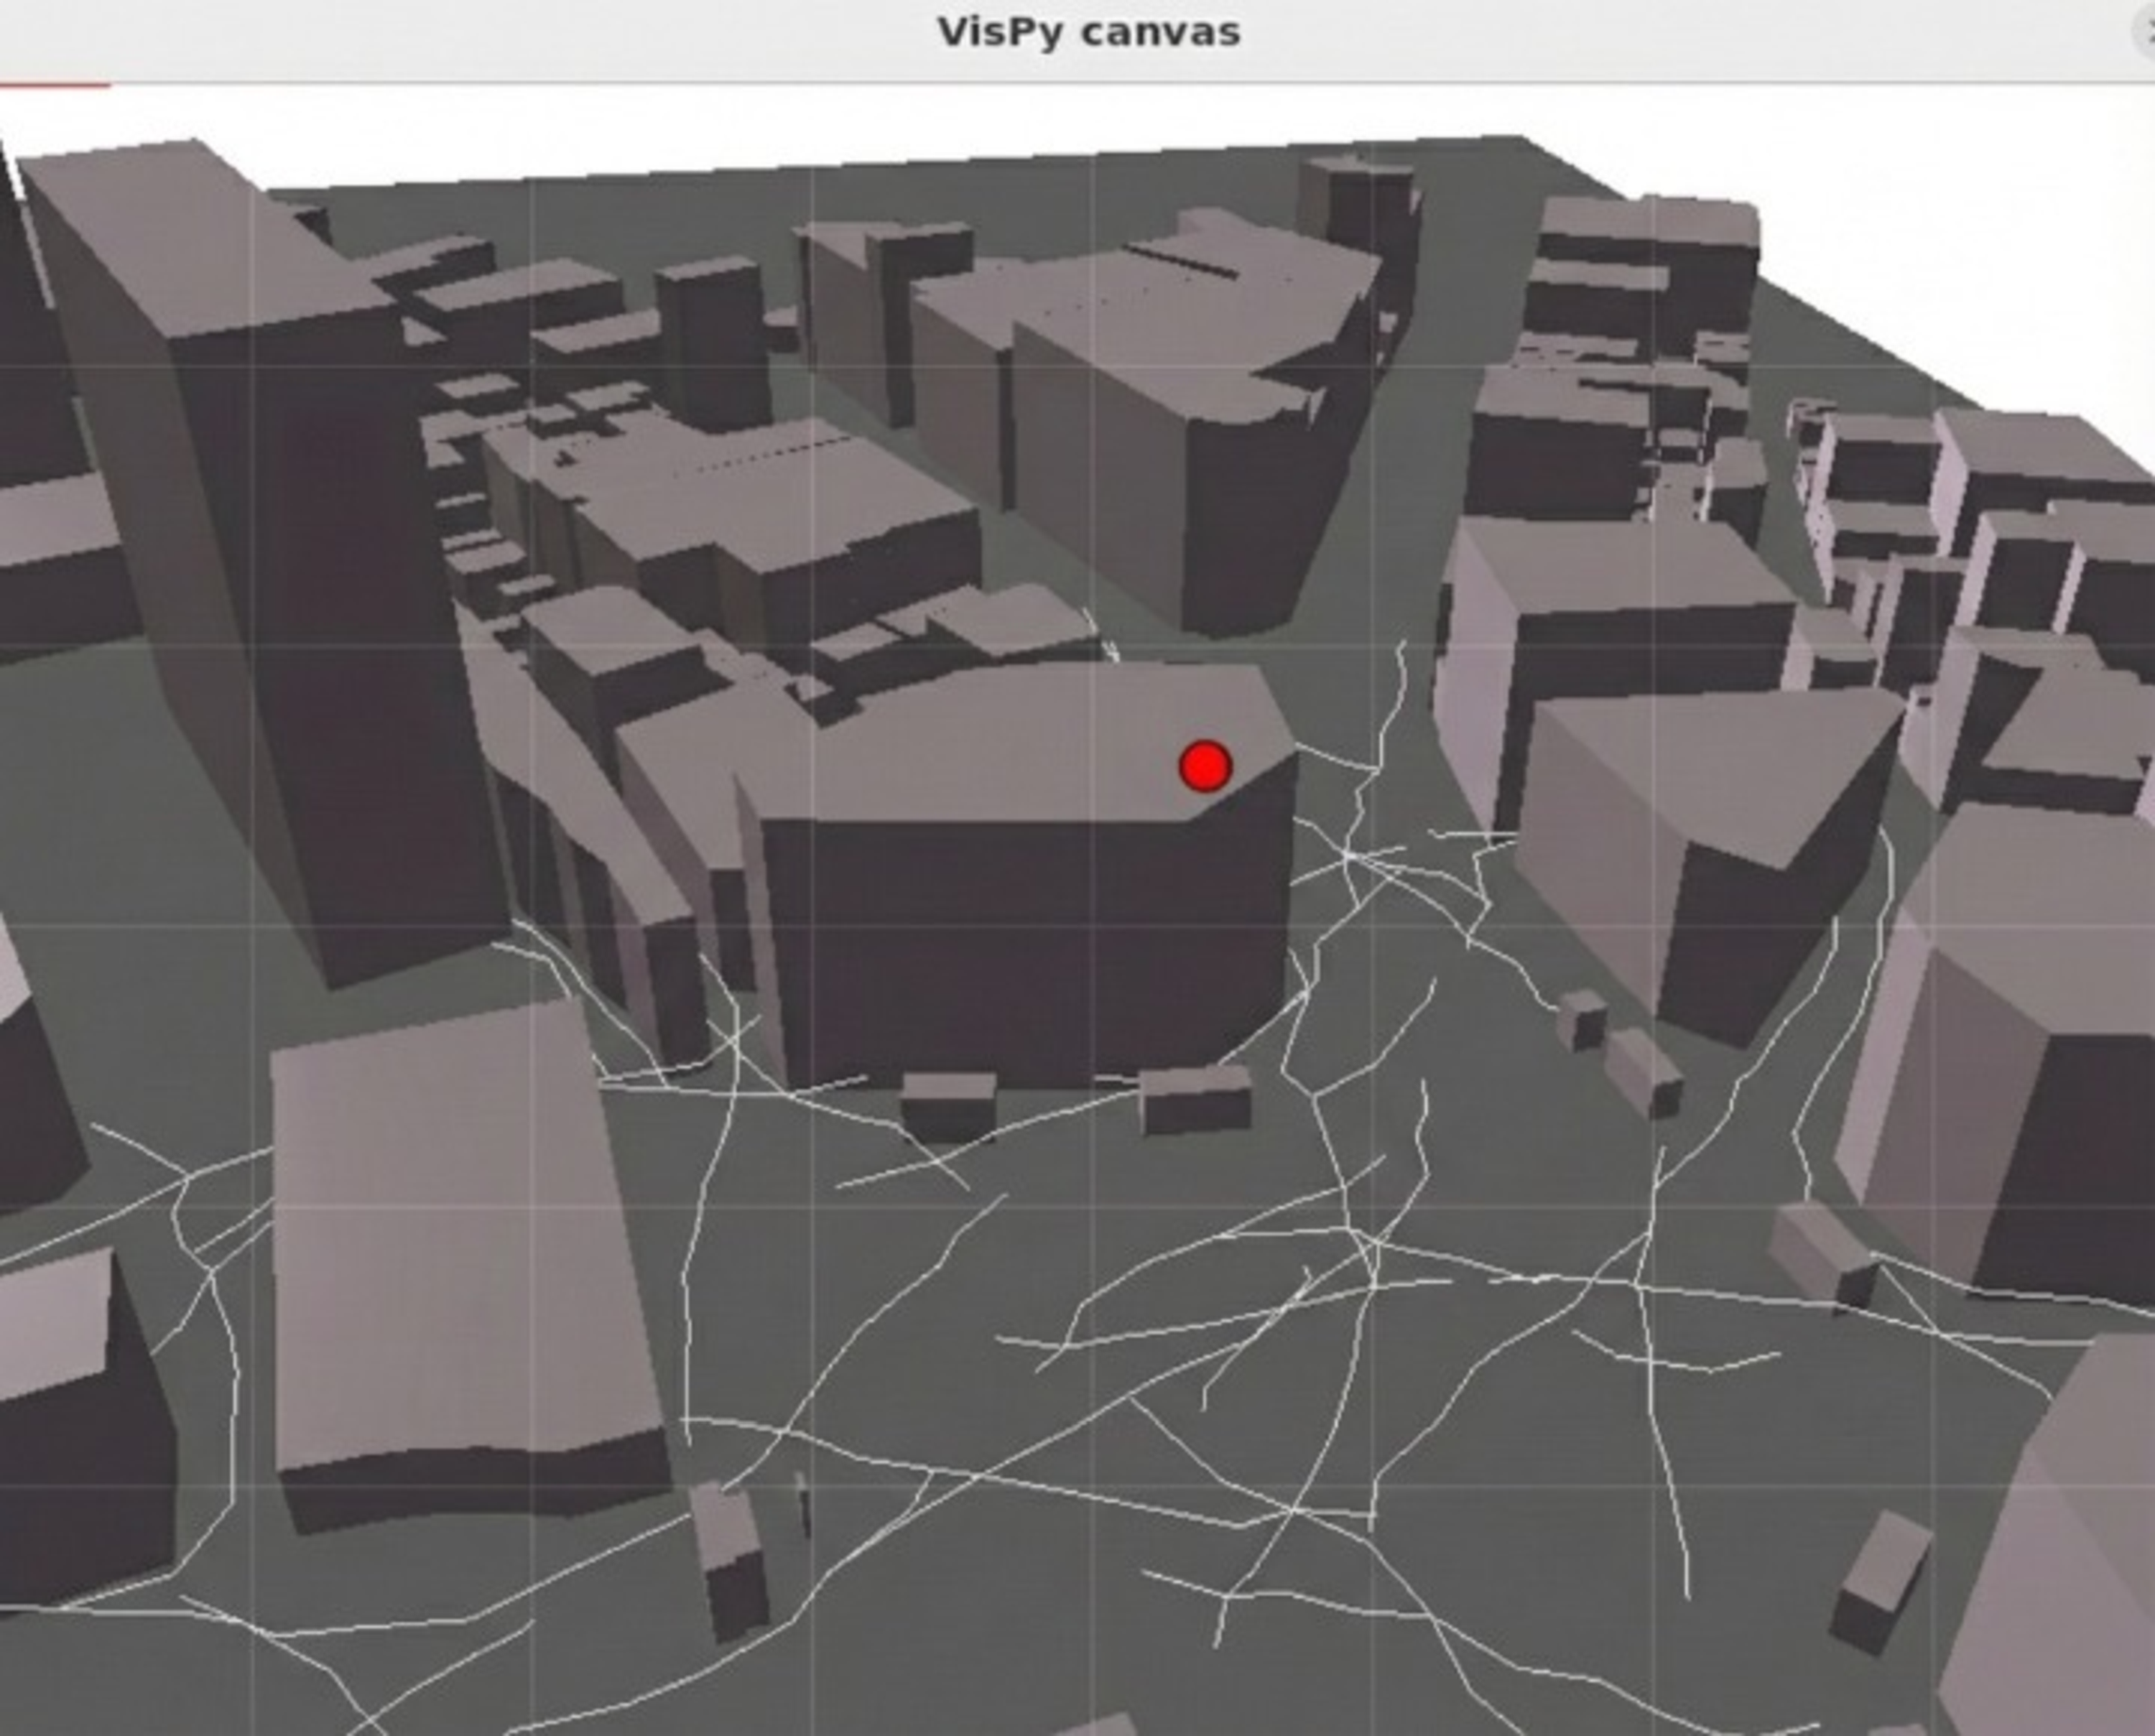
\includegraphics[width=\textwidth]{../picture/4nd/shibuya_2.png}
    \caption{渋谷(詳細2)}
    \label{fig:shibuya_2}
  \end{subfigure}

  \vspace{2mm}
  \begin{subfigure}{0.8\textwidth}
    \centering
    \includegraphics[width=\textwidth]{../picture/4nd/shibuya_fukan.png}
    \caption{渋谷(俯瞰)}
    \label{fig:shibuya_fukan}
  \end{subfigure}
  \caption{三次元モデル化に用いたエリア(渋谷)}
  \label{fig:area_shibuya}
\end{figure}

\begin{figure}[H]
  \centering
  \begin{subfigure}{0.49\textwidth}
    \centering
    \includegraphics[width=\textwidth]{../picture/4nd/shinjuku_1.png}
    \caption{新宿(詳細1)}
    \label{fig:shinjuku_1}
  \end{subfigure}
  \hfill
  \begin{subfigure}{0.49\textwidth}
    \centering
    \includegraphics[width=\textwidth]{../picture/4nd/shinjuku_2.png}
    \caption{新宿(詳細2)}
    \label{fig:shinjuku_2}
  \end{subfigure}
 
  \vspace{2mm}
  \begin{subfigure}{0.8\textwidth}
    \centering
    \includegraphics[width=\textwidth]{../picture/4nd/shinjuku_fukan.png}
    \caption{新宿(俯瞰)}
    \label{fig:shinjuku_fukan}
  \end{subfigure}
  \caption{三次元モデル化に用いたエリア(新宿)}
  \label{fig:area_shinjuku}
\end{figure}

\begin{figure}[H]
  \centering
  \begin{subfigure}{0.8\textwidth}
    \centering
    \includegraphics[width=\textwidth]{../picture/4nd/kinshityou.png}
    \caption{錦糸町(詳細)}
    \label{fig:kinshityou}
  \end{subfigure}

  \vspace{2mm}
  \begin{subfigure}{0.8\textwidth}
    \centering
    \includegraphics[width=\textwidth]{../picture/4nd/kinshityou_fukan.png}
    \caption{錦糸町(俯瞰)}
    \label{fig:kinshityou_fukan}
  \end{subfigure}
  \caption{三次元モデル化に用いたエリア(錦糸町)}
  \label{fig:area_kinshityou}
\end{figure}

\begin{figure}[H]
  \centering
  \begin{subfigure}{0.49\textwidth}
    \centering
    \includegraphics[width=\textwidth]{../picture/4nd/marunouchi_before_build.png}
    \caption{八重洲(ビル建設前)}
    \label{fig:marunouchi_before_build}
  \end{subfigure}
  \hfill
  \begin{subfigure}{0.49\textwidth}
    \centering
    \includegraphics[width=\textwidth]{../picture/4nd/marunouchi_built.png}
    \caption{八重洲(ビル建設後)}
    \label{fig:marunouchi_built}
  \end{subfigure}

  \vspace{2mm}
  \begin{subfigure}{0.8\textwidth}
    \centering
    \includegraphics[width=\textwidth]{../picture/4nd/marunouchi_fukan.png}
    \caption{八重洲(俯瞰)}
    \label{fig:marunouchi_fukan}
  \end{subfigure}
  \caption{三次元モデル化に用いたエリア(八重洲)}
  \label{fig:area_marunouchi}
\end{figure}









レイトレーシングの設定として用いたパラメータを示す.
建物には鉄の物性値を,地面には土の物性値を割り当てた.

\begin{align}
  \text{中心周波数:}\texttt{frequency} &= 3.5~\mathrm{GHz} \\
  \text{サブキャリア間隔:}\texttt{SCS} &= 15~\mathrm{kHz} \\
  \text{帯域幅:}\texttt{bandwidth} &= 20~\mathrm{MHz} \\
  \text{送信アンテナ数:}\texttt{numTx} &= 16 \\
  \text{受信アンテナ数:}\texttt{numRx} &= 2 \\
  \text{速度:}\texttt{velocity} &= 2~\mathrm{km/h},\,20~\mathrm{km/h} \\
  \text{サンプリング周波数:}\texttt{sampling\_frequency} &= 200~\mathrm{Hz} \\
  \text{最大反射回数:}\texttt{max\_reflections} &= 5 \\
  \text{基地局アンテナ縦方向素子間隔:}\texttt{base\_station\_antenna\_vertical\_spacing} &= 0.5 \\
  \text{基地局アンテナ横方向素子間隔:}\texttt{base\_station\_antenna\_horizontal\_spacing} &= 0.5 \\
  \text{端末アンテナ列数:}\texttt{user\_antenna\_rows} &= 2 \\
  \text{端末アンテナ行数:}\texttt{user\_antenna\_cols} &= 1 \\
  \text{端末アンテナ縦方向素子間隔:}\texttt{user\_antenna\_vertical\_spacing} &= 0.5 \\
  \text{端末アンテナ横方向素子間隔:}\texttt{user\_antenna\_horizontal\_spacing} &= 0.5 \\
  \text{反射:}\texttt{reflection} &= \texttt{true} \\
  \text{回折:}\texttt{diffraction} &= \texttt{true} \\
  \text{散乱:}\texttt{scattering} &= \texttt{false} \\
  \text{パス数上限:}\texttt{cir\_num\_paths} &= 200 \\
  \text{遅延の正規化:}\texttt{path.normalize\_delays} &= \texttt{true} \\
  \text{CIRからOFDMへの変換時の正規化:}\texttt{cir\_to\_ofdm\_normalize} &= \texttt{false}
\end{align}

上記の設定より,SRS送信間隔\texttt{srs\_sampling}は
\begin{equation}
  \texttt{srs\_sampling}=\frac{1}{\texttt{sampling\_frequency}}=\frac{1}{200~\mathrm{Hz}}=5~\mathrm{ms}
\end{equation}
となる.


SRSは周波数方向に一定間隔で配置されるとし,SRSが配置された周波数点においてCSIを算出する.
周波数方向のリソースブロック Resource Block, RBは,サブキャリア12本を束ねた単位であり,1RBの周波数幅は
\begin{equation}
  B_{\mathrm{RB}}=12\,SCS=12\times 15~\mathrm{kHz}=180~\mathrm{kHz}
\end{equation}
である.
本研究では,周波数方向に2RBおきにSRSを送信すると仮定する.すなわち,SRSが配置されるRBの間隔は
\begin{equation}
  B_{\mathrm{SRS}}=2\,B_{\mathrm{RB}}=360~\mathrm{kHz}
\end{equation}
である.このとき,CSIはSRSが配置されたRBで算出されるため,周波数方向のCSI系列は2RB間隔でサンプリングされたものとなる.

帯域端の影響を避けるため,本研究では帯域内の中心部分のみを用い,有効なRB数を\(N_{\mathrm{RB}}=96\)とする.
このとき,有効帯域幅は
\begin{equation}
  bandwidth_{\mathrm{eff}}=N_{\mathrm{RB}}\,B_{\mathrm{RB}}=96\times 180~\mathrm{kHz}=17.28~\mathrm{MHz}
\end{equation}
となる.2RBおきにSRSが配置されるため,CSIが算出されるRB数は
\begin{equation}
  N_{\mathrm{rb}}=\frac{N_{\mathrm{RB}}}{2}=\frac{96}{2}=48
\end{equation}
となる.以上より,帯域幅20~MHzでは1スロットあたり周波数方向に\(N_{\mathrm{rb}}=48\)個のRBでCSIが算出される.
以上の条件でレイトレーシングを実行し生成したCSI系列を[時間,リソースブロック,送信アンテナ,受信アンテナ,複素数次元]として保存する.



\subsection{シミュレーション条件}
\label{subsec:simulation_conditions}

本節では,補間手法評価のためのシミュレーション方法について述べる.
補間精度の評価には,第\ref{subsec:terrain_raytracing}節で述べた錦糸町および丸の内の2種類の地形データに対してレイトレーシングにより生成したCSI系列を用いる.
補間手法としては,第\ref{sec:interpolation_methods}節で述べた線形補間,スプライン補間,低次多項式近似,ニューラルネットワーク補間を比較対象とする.
ニューラルネットワーク補間器の学習には,評価対象とは異なる地形データから生成したCSI系列を用いる.
錦糸町駅前のCSI系列を補間するモデルは,新宿,池袋,渋谷の3地点から生成したCSI系列で学習する.
丸の内駅前のCSI系列を補間するモデルは,丸の内駅前から生成したCSI系列を学習データとして用いる.
前者は他セルで運用していた補間器を新規基地局へ展開する状況を想定しており,後者は同一セル内で環境変動が生じた際に補間器を再学習する状況を想定している.

補間器の構成は第\ref{sec:interpolation_methods}節で述べたMLPであり,$\mathrm{Linear}(6F\rightarrow 2048)\rightarrow \mathrm{ReLU}\rightarrow\mathrm{Linear}(2048\rightarrow 1024)\rightarrow \mathrm{ReLU}\rightarrow\mathrm{Linear}(1024\rightarrow F)$の3層構造とする.
学習時の損失関数には補間値$\widetilde{\bm{H}}_t$と真値$\bm{H}_t$の平均二乗誤差を用い,最適化にはAdamを使用する.
学習率は$10^{-4}$,バッチサイズは128,エポック数は10とする.

パイロット信号の送信周期が変化した場合における補間精度を評価するため,推定値と予測対象の割合を変化させた複数の観測パターンを設定する.
観測パターンは,周期$P$の文字列として$\mathrm{S}$を観測時刻,$\mathrm{P}$を欠損時刻として定義し,以下の3種類を用いる.
\begin{align}
\text{SSSP} &: \; \mathrm{S},\mathrm{S},\mathrm{S},\mathrm{P} \; \text{を周期 }P=4\text{で繰り返し} \\
\text{SSP}  &: \; \mathrm{S},\mathrm{S},\mathrm{P} \; \text{を周期 }P=3\text{で繰り返し} \\
\text{SP}   &: \; \mathrm{S},\mathrm{P} \; \text{を周期 }P=2\text{で繰り返し}
\end{align}
SSSPでは4スロットに1回,SSPでは3スロットに1回,SPでは2スロットに1回の頻度で欠損が発生する.
観測パターンに応じて欠損率が25\%から50\%まで変化するため,各パターンにおいて有効な補間手法を特定する.
補間対象となる時刻集合$\mathcal{T}_P$は$\mathcal{T}_P \triangleq \{t \mid t \bmod P = P-1\}$として定義し,観測時刻集合は$\mathcal{T}_S=\{0,1,\dots,T-1\}\setminus\mathcal{T}_P$とする.

評価指標には正規化平均二乗誤差NMSEを用いる.
補間対象時刻$t\in\mathcal{T}_P$における補間値$\widetilde{\bm{H}}_t$と真値$\bm{H}_t$の誤差を
\begin{equation}
  \mathrm{NMSE}(t)
  =\frac{\left\lVert \widetilde{\bm{H}}_t-\bm{H}_t\right\rVert_2^2}{\left\lVert \bm{H}_t\right\rVert_2^2}
  \label{eq:nmse_interp}
\end{equation}
として定義する.
全ファイルおよび全補間対象時刻に対してNMSEを算出し,その平均値
\begin{equation}
\overline{\mathrm{NMSE}}
=
\frac{1}{N}\sum_{n=1}^{N}\mathrm{NMSE}(t_n)
\end{equation}
を最終的な評価スコアとする.ここで$N$は評価に用いた補間対象時刻の総数である.



\section{地形ごとの補間手法比較評価}

\subsection{結果}
本節では,各地形データから生成したCSI系列に対する補間精度の評価結果を示す.
評価はSSSPパターンを用いて実施し,各補間手法のNMSEを比較する.

\subsubsection{錦糸町データセットにおける補間精度}
錦糸町駅前の地形データから生成した284ファイルのCSI系列に対する補間精度評価を表\ref{tab:kinshicho_sssp_results}に示す.
多項式近似の設定において,次数と片側近傍点数を記載する.例えば「4次,片側3点ずつ」は4次多項式を用い,補間対象時刻の前後それぞれ3点ずつ,計6点の推定値を近傍として使用することを意味する.
ニューラルネットワーク補間の設定において,$c$はコンテキストサイズを表す.

\begin{table}[H]
  \centering
  \caption{錦糸町データセットにおけるSSSPパターンの補間精度}
  \label{tab:kinshicho_sssp_results}
  \begin{tabular}{llc}
    \hline
    手法 & 設定 & NMSE \\
    \hline
    線形補間 & -- & 0.3748 \\
    スプライン補間 & -- & \textbf{0.0061} \\
    多項式近似 & 2次,片側3点ずつ & 0.0517 \\
    多項式近似 & 3次,片側3点ずつ & 0.0517 \\
    多項式近似 & 4次,片側3点ずつ & \textbf{0.0059} \\
    多項式近似 & 5次,片側3点ずつ & \textbf{0.0059} \\
    多項式近似 & 6次,片側3点ずつ & 0.1432 \\
    多項式近似 & 4次,片側6点ずつ & 0.2288 \\
    多項式近似 & 4次,片側9点ずつ & 0.2584 \\
    ニューラルネットワーク補間 & $c=1$ & 0.3853 \\
    ニューラルネットワーク補間 & $c=2$ & 0.5112 \\
    ニューラルネットワーク補間 & $c=3$ & 0.4737 \\
    \hline
  \end{tabular}
\end{table}

スプライン補間および4次または5次の多項式近似がNMSE 0.006程度で最良の精度を達成した.
一方,線形補間やニューラルネットワーク補間はNMSE 0.37以上と低い精度にとどまった.
ニューラルネットワークが低精度となった要因として,学習データが錦糸町と異なる3地点で構成されているため,チャネル特性の違いに対応できなかったことが考えられる.





\subsubsection{丸の内(LoS)データセットにおける補間精度}
丸の内(LoS)の地形データから生成した101ファイルのCSI系列に対する補間精度評価を表\ref{tab:marunouchi_sssp_results}に示す.

\begin{table}[H]
  \centering
  \caption{丸の内(LoS)データセットにおけるSSSPパターンの補間精度}
  \label{tab:marunouchi_sssp_results}
  \begin{tabular}{llc}
    \hline
    手法 & 設定 & NMSE \\
    \hline
    線形補間 & -- & 0.1644 \\
    スプライン補間 & -- & \textbf{0.0456} \\
    多項式近似 & 2次,片側3点ずつ & 0.0576 \\
    多項式近似 & 3次,片側3点ずつ & 0.0576 \\
    多項式近似 & 4次,片側3点ずつ & \textbf{0.0463} \\
    多項式近似 & 5次,片側3点ずつ & \textbf{0.0463} \\
    多項式近似 & 6次,片側3点ずつ & 0.1517 \\
    多項式近似 & 4次,片側6点ずつ & 0.1517 \\
    多項式近似 & 4次,片側9点ずつ & 0.1571 \\
    ニューラルネットワーク補間 & $c=1$ & 0.1453 \\
    ニューラルネットワーク補間 & $c=2$ & 0.1314 \\
    ニューラルネットワーク補間 & $c=3$ & 0.4911 \\
    \hline
  \end{tabular}
\end{table}

丸の内(NLoS)データセットに対するSSSPパターンの補間精度評価を表\ref{tab:marunouchi_nlos_sssp_results}に示す.
丸の内(NLoS)データセットの評価では,線形補間およびニューラルネットワーク補間を比較対象から除外した.
錦糸町および丸の内(LoS)データセットの評価において,線形補間は補間対象の前後1点のみを用いる単純な手法であり,NMSEが0.16から0.37と低精度であることが確認された.
ニューラルネットワーク補間も学習データと評価データの地点差に起因するドメインシフトにより解析的手法を下回る精度にとどまった.
これらの結果から,丸の内(NLoS)データセットにおいても同様の傾向が予想されるため,評価対象から除外した.

\begin{table}[H]
  \centering
  \caption{丸の内(NLoS)データセットにおけるSSSPパターンの補間精度}
  \label{tab:marunouchi_nlos_sssp_results}
  \begin{tabular}{llc}
    \hline
    手法 & 設定 & NMSE \\
    \hline
    スプライン補間 & -- & \textbf{0.057395} \\
    多項式近似 & 2次,片側3点ずつ & 0.082413 \\
    多項式近似 & 3次,片側3点ずつ & 0.082413 \\
    多項式近似 & 4次,片側3点ずつ & 0.057968 \\
    多項式近似 & 5次,片側3点ずつ & 0.057968 \\
    多項式近似 & 6次,片側3点ずつ & 0.173984 \\
    多項式近似 & 4次,片側6点ずつ & 0.213839 \\
    多項式近似 & 4次,片側9点ずつ & 0.224907 \\
    \hline
  \end{tabular}
\end{table}

丸の内(LoS)データセットにおいても,スプライン補間と4次または5次の多項式近似が最良の精度を示し,NMSEは0.04から0.05程度であった.
ニューラルネットワーク補間の精度は錦糸町データセットと比較して向上している.これは,丸の内(LoS)データセットでは学習と評価が同一地点のCSI系列で構成されているためである.
両データセットを通じて,スプライン補間と4次多項式近似が一貫して高い補間精度を達成した.
多項式近似では,次数4と次数5で同一のNMSEを示した.これは総近傍点数$K=6$($k=3$)に対して次数5の多項式が過剰適合となり,事実上4次と同等の近似となったためと考えられる.
次数6では精度が大幅に低下しており,過学習による悪影響が確認された.
近傍点数を増やした場合においても精度が低下しており,補間対象から離れた時刻の推定値は精度向上に寄与しないことが示された.


\section{パイロット疎化拡大時の補間精度評価}
本節では,パイロット信号の送信頻度をさらに低減した場合の補間精度を評価する.
前節ではSSSPパターンを用いて評価したが,本節ではSSPパターンおよびSPパターンを追加し,欠損率が33\%および50\%に増加した場合の補間精度を比較する.

\subsection{結果}

\subsubsection{錦糸町データセットにおける補間精度}
錦糸町データセットに対するSSPパターンおよびSPパターンの補間精度評価を表\ref{tab:kinshicho_ssp_sp_results}に示す.

\begin{table}[H]
  \centering
  \caption{錦糸町データセットにおけるSSPおよびSPパターンの補間精度}
  \label{tab:kinshicho_ssp_sp_results}
  \begin{tabular}{llrr}
    \hline
    手法 & 設定 & SSP & SP \\
    \hline
    線形補間 & -- & 0.2751 & 0.2865 \\
    スプライン補間 & -- & \textbf{0.0062} & \textbf{0.0130} \\
    多項式近似 & 2次,片側3点ずつ & 0.1174 & 0.1757 \\
    多項式近似 & 3次,片側3点ずつ & 0.1174 & 0.1757 \\
    多項式近似 & 4次,片側3点ずつ & \textbf{0.0069} & \textbf{0.0162} \\
    多項式近似 & 5次,片側3点ずつ & \textbf{0.0069} & \textbf{0.0162} \\
    多項式近似 & 6次,片側3点ずつ & 0.1588 & 0.2184 \\
    多項式近似 & 4次,片側6点ずつ & 0.1627 & 0.2242 \\
    多項式近似 & 4次,片側9点ずつ & 0.2795 & 0.3130 \\
    ニューラルネットワーク補間 & $c=1$ & 0.3121 & 0.3781 \\
    ニューラルネットワーク補間 & $c=2$ & 0.4268 & 0.3968 \\
    ニューラルネットワーク補間 & $c=3$ & 0.5761 & 0.5961 \\
    \hline
  \end{tabular}
\end{table}

SSPパターンにおいても,スプライン補間と4次多項式近似が最良の精度を示し,NMSEは0.006から0.007程度であった.
SPパターンでは欠損率が50\%に達するが,スプライン補間と4次多項式近似はNMSE 0.013から0.016程度を維持した.
ニューラルネットワーク補間は全パターンで0.3以上のNMSEとなり,学習データと評価データの地点差による汎化性能の低さが確認された.

以降のSPP/SPPPパターンの評価では,線形補間およびニューラルネットワーク補間を比較対象から除外した.
SSSP/SSP/SPパターンの評価において,線形補間はNMSEが0.16から0.37と低精度であり,補間対象の前後1点のみを用いる単純な手法では時間変動を十分に捉えられないことが確認された.
ニューラルネットワーク補間も同様に精度が低く,学習データと評価データの地点差に起因するドメインシフトにより,スプライン補間や多項式近似といった解析的手法を下回る結果となった.
連続補間パターンでは単一フレーム補間よりも推定が困難であり,これらの手法の精度低下が予想されるため,評価対象から除外した.

\noindent
錦糸町データセットに対するSPPパターン(周期3,2フレーム連続補間)およびSPPPパターン(周期4,3フレーム連続補間)の補間精度評価をそれぞれ表\ref{tab:kinshicho_spp_results}および表\ref{tab:kinshicho_sppp_results}に示す.
本実験では補間位置が複数存在するため,補間位置ごとのNMSE(pos)と,それらを統合したOverall NMSEを算出した.

\begin{table}[H]
  \centering
  \caption{錦糸町データセットにおけるSPPパターン(周期3,2フレーム連続補間)の補間精度}
  \label{tab:kinshicho_spp_results}
  \begin{tabular}{llrrr}
    \hline
    手法 & 設定 & Overall NMSE & pos0 & pos1 \\
    \hline
    多項式近似 & 5次,片側3点ずつ & \textbf{0.1286} & 0.1283 & 0.1288 \\
    スプライン補間 & 片側3点ずつ & 0.1314 & 0.1311 & 0.1317 \\
    スプライン補間 & 片側6点ずつ & 0.1364 & 0.1361 & 0.1366 \\
    スプライン補間 & 片側9点ずつ & 0.1364 & 0.1361 & 0.1367 \\
    多項式近似 & 4次,片側3点ずつ & 0.1691 & 0.1690 & 0.1691 \\
    多項式近似 & 3次,片側3点ずつ & 0.2453 & 0.2456 & 0.2449 \\
    多項式近似 & 2次,片側3点ずつ & 0.2491 & 0.2497 & 0.2485 \\
    多項式近似 & 6次,片側6点ずつ & 0.2650 & 0.2654 & 0.2646 \\
    多項式近似 & 5次,片側6点ずつ & 0.3092 & 0.3096 & 0.3088 \\
    多項式近似 & 4次,片側6点ずつ & 0.3116 & 0.3122 & 0.3110 \\
    多項式近似 & 6次,片側9点ずつ & 0.3366 & 0.3372 & 0.3360 \\
    多項式近似 & 5次,片側9点ずつ & 0.3709 & 0.3714 & 0.3705 \\
    多項式近似 & 4次,片側9点ずつ & 0.3711 & 0.3718 & 0.3703 \\
    多項式近似 & 6次,片側3点ずつ & 0.4187 & 0.4188 & 0.4186 \\
    \hline
  \end{tabular}
\end{table}

\begin{table}[H]
  \centering
  \caption{錦糸町データセットにおけるSPPPパターン(周期4,3フレーム連続補間)の補間精度}
  \label{tab:kinshicho_sppp_results}
  \begin{tabular}{llrrrr}
    \hline
    手法 & 設定 & Overall NMSE & pos0 & pos1 & pos2 \\
    \hline
    多項式近似 & 5次,片側3点ずつ & \textbf{0.2756} & 0.2088 & 0.4091 & 0.2088 \\
    スプライン補間 & 片側3点ずつ & 0.2822 & 0.2128 & 0.4209 & 0.2129 \\
    スプライン補間 & 片側6点ずつ & 0.2830 & 0.2134 & 0.4219 & 0.2136 \\
    スプライン補間 & 片側9点ずつ & 0.2830 & 0.2134 & 0.4218 & 0.2136 \\
    多項式近似 & 4次,片側3点ずつ & 0.3359 & 0.2992 & 0.4091 & 0.2993 \\
    多項式近似 & 3次,片側3点ずつ & 0.3454 & 0.3236 & 0.3895 & 0.3230 \\
    多項式近似 & 6次,片側6点ずつ & 0.3518 & 0.3381 & 0.3800 & 0.3372 \\
    多項式近似 & 2次,片側3点ずつ & 0.3652 & 0.3537 & 0.3895 & 0.3525 \\
    多項式近似 & 5次,片側6点ずつ & 0.3652 & 0.3599 & 0.3755 & 0.3604 \\
    多項式近似 & 4次,片側6点ずつ & 0.3708 & 0.3687 & 0.3755 & 0.3683 \\
    多項式近似 & 6次,片側9点ずつ & 0.3787 & 0.3769 & 0.3828 & 0.3764 \\
    多項式近似 & 5次,片側9点ずつ & 0.4033 & 0.4016 & 0.4054 & 0.4028 \\
    多項式近似 & 4次,片側9点ずつ & 0.4041 & 0.4035 & 0.4054 & 0.4035 \\
    多項式近似 & 6次,片側3点ずつ & 0.5047 & 0.3987 & 0.7272 & 0.3880 \\
    \hline
  \end{tabular}
\end{table}





\subsubsection{丸の内(LoS)データセットにおける補間精度}
丸の内(LoS)データセットに対するSSPパターンおよびSPパターンの補間精度評価を表\ref{tab:marunouchi_ssp_sp_results}に示す.

\begin{table}[H]
  \centering
  \caption{丸の内(LoS)データセットにおけるSSPおよびSPパターンの補間精度}
  \label{tab:marunouchi_ssp_sp_results}
  \begin{tabular}{llrr}
    \hline
    手法 & 設定 & SSP & SP \\
    \hline
    線形補間 & -- & 0.1380 & 0.1474 \\
    スプライン補間 & -- & \textbf{0.0278} & \textbf{0.0360} \\
    多項式近似 & 2次,片側3点ずつ & 0.0969 & 0.1177 \\
    多項式近似 & 3次,片側3点ずつ & 0.0969 & 0.1177 \\
    多項式近似 & 4次,片側3点ずつ & \textbf{0.0278} & \textbf{0.0370} \\
    多項式近似 & 5次,片側3点ずつ & \textbf{0.0278} & \textbf{0.0370} \\
    多項式近似 & 6次,片側3点ずつ & 0.1638 & 0.2244 \\
    多項式近似 & 4次,片側6点ずつ & 0.1070 & 0.1324 \\
    多項式近似 & 4次,片側9点ずつ & 0.1326 & 0.1431 \\
    ニューラルネットワーク補間 & $c=1$ & 0.1401 & 0.1424 \\
    ニューラルネットワーク補間 & $c=2$ & 0.1967 & 0.1658 \\
    ニューラルネットワーク補間 & $c=3$ & 0.1743 & 0.2269 \\
    \hline
  \end{tabular}
\end{table}





\noindent
丸の内(LoS)データセットに対するSPPパターン(周期3,2フレーム連続補間)およびSPPPパターン(周期4,3フレーム連続補間)の補間精度評価をそれぞれ表\ref{tab:marunouchi_los_spp_results}および表\ref{tab:marunouchi_los_sppp_results}に示す.
本実験では補間位置が複数存在するため,補間位置ごとのNMSE(pos)と,それらを統合したOverall NMSEを算出した.

\begin{table}[H]
  \centering
  \caption{丸の内(LoS)データセットにおけるSPPパターン(周期3,2フレーム連続補間)の補間精度}
  \label{tab:marunouchi_los_spp_results}
  \begin{tabular}{llrrr}
    \hline
    手法 & 設定 & Overall NMSE & pos0 & pos1 \\
    \hline
    多項式近似 & 5次,片側3点ずつ & \textbf{0.1675} & 0.1645 & 0.1706 \\
    スプライン補間 & 片側3点ずつ & 0.1742 & 0.1712 & 0.1773 \\
    スプライン補間 & 片側6点ずつ & 0.1756 & 0.1756 & 0.1756 \\
    スプライン補間 & 片側9点ずつ & 0.1757 & 0.1757 & 0.1757 \\
    多項式近似 & 3次,片側3点ずつ & 0.1793 & 0.1792 & 0.1794 \\
    多項式近似 & 6次,片側6点ずつ & 0.1827 & 0.1826 & 0.1829 \\
    多項式近似 & 2次,片側3点ずつ & 0.1845 & 0.1807 & 0.1884 \\
    多項式近似 & 4次,片側3点ずつ & 0.1992 & 0.1908 & 0.2076 \\
    多項式近似 & 5次,片側6点ずつ & 0.2251 & 0.2252 & 0.2250 \\
    多項式近似 & 4次,片側6点ずつ & 0.2260 & 0.2258 & 0.2262 \\
    多項式近似 & 6次,片側9点ずつ & 0.2262 & 0.2261 & 0.2263 \\
    多項式近似 & 4次,片側9点ずつ & 0.2566 & 0.2565 & 0.2567 \\
    多項式近似 & 5次,片側9点ずつ & 0.2566 & 0.2567 & 0.2566 \\
    多項式近似 & 6次,片側3点ずつ & 0.4523 & 0.4524 & 0.4521 \\
    \hline
  \end{tabular}
\end{table}

\begin{table}[H]
  \centering
  \caption{丸の内(LoS)データセットにおけるSPPPパターン(周期4,3フレーム連続補間)の補間精度}
  \label{tab:marunouchi_los_sppp_results}
  \begin{tabular}{llrrrr}
    \hline
    手法 & 設定 & Overall NMSE & pos0 & pos1 & pos2 \\
    \hline
    多項式近似 & 5次,片側3点ずつ & \textbf{0.2565} & 0.2039 & 0.3600 & 0.2057 \\
    スプライン補間 & 片側6点ずつ & 0.2615 & 0.2088 & 0.3696 & 0.2061 \\
    スプライン補間 & 片側9点ずつ & 0.2617 & 0.2090 & 0.3698 & 0.2062 \\
    スプライン補間 & 片側3点ずつ & 0.2618 & 0.2079 & 0.3682 & 0.2092 \\
    多項式近似 & 3次,片側3点ずつ & 0.2717 & 0.2441 & 0.3236 & 0.2474 \\
    多項式近似 & 5次,片側6点ずつ & 0.2761 & 0.2614 & 0.3068 & 0.2601 \\
    多項式近似 & 4次,片側6点ずつ & 0.2813 & 0.2687 & 0.3068 & 0.2684 \\
    多項式近似 & 6次,片側9点ずつ & 0.2868 & 0.2754 & 0.3097 & 0.2753 \\
    多項式近似 & 2次,片側3点ずつ & 0.2871 & 0.2645 & 0.3236 & 0.2732 \\
    多項式近似 & 6次,片側6点ずつ & 0.2879 & 0.2645 & 0.3353 & 0.2641 \\
    多項式近似 & 4次,片側3点ずつ & 0.2907 & 0.2470 & 0.3600 & 0.2649 \\
    多項式近似 & 5次,片側9点ずつ & 0.2945 & 0.2893 & 0.3060 & 0.2883 \\
    多項式近似 & 4次,片側9点ずつ & 0.2975 & 0.2933 & 0.3060 & 0.2933 \\
    多項式近似 & 6次,片側3点ずつ & 0.5428 & 0.4325 & 0.7700 & 0.4260 \\
    \hline
  \end{tabular}
\end{table}

丸の内(LoS)データセットにおいても同様の傾向が確認された.
スプライン補間と4次多項式近似はSSPパターンでNMSE 0.03程度,SPパターンでNMSE 0.04程度を達成した.
ニューラルネットワーク補間は錦糸町データセットと比較して精度が向上しており,同一地点での学習による効果が認められる.
ただし,スプライン補間や4次多項式近似には及ばず,学習ベースの補間器が解析的手法を上回る条件は本評価では見出されなかった.







丸の内(NLoS)データセットに対するSSPパターンおよびSPパターンの補間精度評価を表\ref{tab:marunouchi_nlos_ssp_sp_results}に示す.

\begin{table}[H]
  \centering
  \caption{丸の内(NLoS)データセットにおけるSSPおよびSPパターンの補間精度}
  \label{tab:marunouchi_nlos_ssp_sp_results}
  \begin{tabular}{llrr}
    \hline
    手法 & 設定 & SSP & SP \\
    \hline
    スプライン補間 & 片側3点ずつ & 0.054962 & \textbf{0.053230} \\
    多項式近似 & 2次,片側3点ずつ & 0.134070 & 0.170361 \\
    多項式近似 & 3次,片側3点ずつ & 0.134070 & 0.170361 \\
    多項式近似 & 4次,片側3点ずつ & \textbf{0.054486} & 0.054971 \\
    多項式近似 & 5次,片側3点ずつ & \textbf{0.054486} & 0.054971 \\
    多項式近似 & 6次,片側3点ずつ & 0.189349 & 0.249500 \\
    多項式近似 & 4次,片側6点ずつ & 0.159744 & 0.193791 \\
    多項式近似 & 4次,片側9点ずつ & 0.217653 & 0.280060 \\
    \hline
  \end{tabular}
\end{table}

\noindent
丸の内(NLoS)データセットに対するSPPパターン(周期3,2フレーム連続補間)およびSPPPパターン(周期4,3フレーム連続補間)の補間精度評価をそれぞれ表\ref{tab:marunouchi_nlos_spp_results}および表\ref{tab:marunouchi_nlos_sppp_results}に示す.
本実験では補間位置が複数存在するため,補間位置ごとのNMSE(pos)と,それらを統合したOverall NMSEを算出した.

\begin{table}[H]
  \centering
  \caption{丸の内(NLoS)データセットにおけるSPPパターン(周期3,2フレーム連続補間)の補間精度}
  \label{tab:marunouchi_nlos_spp_results}
  \begin{tabular}{llrrr}
    \hline
    手法 & 設定 & Overall NMSE & pos0 & pos1 \\
    \hline
    多項式近似 & 2次,片側3点ずつ & 0.212486 & 0.212546 & 0.212427 \\
    多項式近似 & 3次,片側3点ずつ & 0.208927 & 0.208889 & 0.208965 \\
    多項式近似 & 4次,片側3点ずつ & 0.182280 & 0.182264 & 0.182297 \\
    多項式近似 & 5次,片側3点ずつ & \textbf{0.152921} & 0.152825 & 0.153017 \\
    多項式近似 & 6次,片側3点ずつ & 0.458041 & 0.458171 & 0.457911 \\
    多項式近似 & 4次,片側6点ずつ & 0.281313 & 0.281317 & 0.281308 \\
    多項式近似 & 5次,片側6点ずつ & 0.278874 & 0.278817 & 0.278931 \\
    多項式近似 & 6次,片側6点ずつ & 0.210491 & 0.210727 & 0.210256 \\
    多項式近似 & 4次,片側9点ずつ & 0.345813 & 0.345677 & 0.345950 \\
    多項式近似 & 5次,片側9点ずつ & 0.345791 & 0.345676 & 0.345906 \\
    多項式近似 & 6次,片側9点ずつ & 0.308767 & 0.308690 & 0.308845 \\
    スプライン補間 & 片側3点ずつ & 0.157235 & 0.157129 & 0.157342 \\
    スプライン補間 & 片側6点ずつ & 0.160927 & 0.160826 & 0.161027 \\
    スプライン補間 & 片側9点ずつ & 0.160998 & 0.160898 & 0.161098 \\
    \hline
  \end{tabular}
\end{table}

\begin{table}[H]
  \centering
  \caption{丸の内(NLoS)データセットにおけるSPPPパターン(周期4,3フレーム連続補間)の補間精度}
  \label{tab:marunouchi_nlos_sppp_results}
  \begin{tabular}{llrrrr}
    \hline
    手法 & 設定 & Overall NMSE & pos0 & pos1 & pos2 \\
    \hline
    多項式近似 & 2次,片側3点ずつ & 0.317059 & 0.305640 & 0.339997 & 0.305541 \\
    多項式近似 & 3次,片側3点ずつ & 0.298134 & 0.277190 & 0.339997 & 0.277216 \\
    多項式近似 & 4次,片側3点ずつ & 0.300981 & 0.267654 & 0.368069 & 0.267219 \\
    多項式近似 & 5次,片側3点ずつ & \textbf{0.261897} & 0.209025 & 0.368069 & 0.208598 \\
    多項式近似 & 6次,片側3点ずつ & 0.548121 & 0.437063 & 0.780505 & 0.426793 \\
    多項式近似 & 4次,片側6点ずつ & 0.361749 & 0.353657 & 0.377893 & 0.353699 \\
    多項式近似 & 5次,片側6点ずつ & 0.357749 & 0.347582 & 0.377893 & 0.347772 \\
    多項式近似 & 6次,片側6点ずつ & 0.324681 & 0.309704 & 0.354742 & 0.309596 \\
    多項式近似 & 4次,片側9点ずつ & 0.376005 & 0.373168 & 0.381733 & 0.373114 \\
    多項式近似 & 5次,片側9点ずつ & 0.374111 & 0.370286 & 0.381733 & 0.370314 \\
    多項式近似 & 6次,片側9点ずつ & 0.361447 & 0.354386 & 0.375723 & 0.354233 \\
    スプライン補間 & 片側3点ずつ & 0.268611 & 0.213832 & 0.378606 & 0.213396 \\
    スプライン補間 & 片側6点ずつ & 0.270807 & 0.215560 & 0.381694 & 0.215167 \\
    スプライン補間 & 片側9点ずつ & 0.270968 & 0.215650 & 0.381976 & 0.215277 \\
    \hline
  \end{tabular}
\end{table}

SSSP/SSP/SPパターンを通じた結果を総括する.
表\ref{tab:summary_all_patterns}に,SSSP/SSP/SPパターンにおける各手法の平均NMSEを示す.

\begin{table}[H]
  \centering
  \caption{SSSP/SSP/SPパターンにおける平均NMSE}
  \label{tab:summary_all_patterns}
  \begin{tabular}{llrrr}
    \hline
    手法 & 設定 & 錦糸町 & 丸の内(LoS) & 丸の内(NLoS) \\
    \hline
    スプライン補間 & -- & 0.0084 & 0.0365 & 0.0552 \\
    多項式近似 & 4次,片側3点ずつ & 0.0097 & 0.0370 & 0.0558 \\
    多項式近似 & 5次,片側3点ずつ & 0.0097 & 0.0370 & 0.0558 \\
    \hline
  \end{tabular}
\end{table}

スプライン補間と4次多項式近似は,パイロット疎化率が25\%から50\%に変化しても安定した補間精度を維持した.
錦糸町では両手法の平均NMSEは0.01以下であり,丸の内(LoS)では0.04以下,丸の内(NLoS)においても0.06未満を維持した.
本評価の結果から,チャネル予測モデルの重み更新に用いる補間手法として,スプライン補間または4次多項式近似が有効であることが示唆された.


\section{おわりに}
本章では,チャネル予測モデルの重み更新に用いる補間手法を選定するため,錦糸町駅前と丸の内駅前の2種類の地形データから生成したCSI系列に対して補間精度の比較実験を実施した.
比較対象として,スプライン補間および多項式近似を用いた.

実験の結果,スプライン補間と4次多項式近似が両データセットで最良の精度を達成し,錦糸町ではNMSEは0.01以下,丸の内では0.04から0.06程度であった.
パイロット信号の送信頻度を低減し欠損率が25\%から50\%に増加した場合においても,両手法は安定した補間精度を維持した.

以上の結果から,次章以降の実験ではスプライン補間または4次多項式近似を用いて提案機構を実装する.
